\documentclass{article}
\usepackage{graphicx}
\usepackage[utf8]{inputenc}

\title{MAC0350 - EP1}
\date{}
\author{
	André Ferrari Moukarzel \\ 9298169
	\and
	Arthur Vieira Barbosa \\ 6482041
	\and
	Gabriel Sarti Massukado \\ 10284177
	\and
	Matheus Lima Cunha \\ 10297755
}

\begin{document}
  \pagenumbering{gobble}
  \maketitle
  \newpage
  \pagenumbering{arabic}
  
  \section{Validação do Modelo}
  
  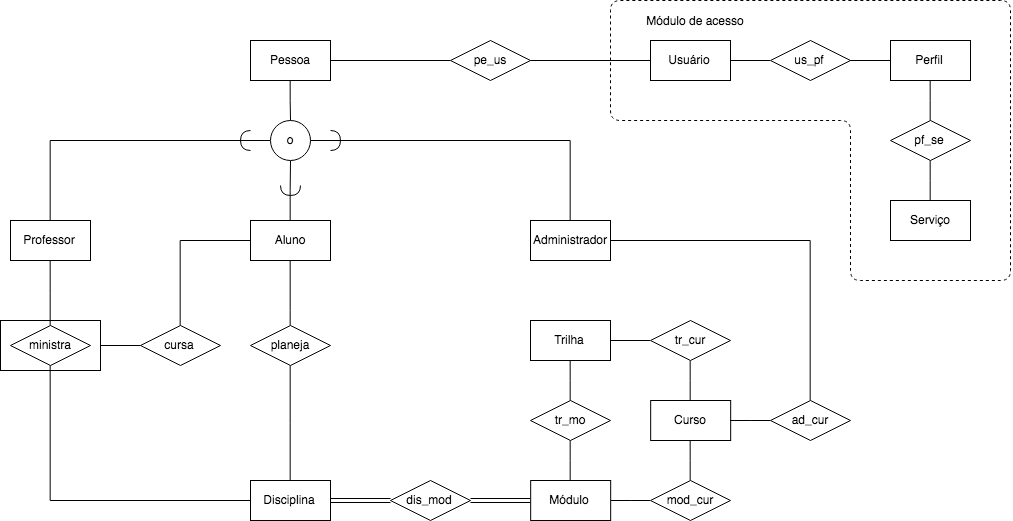
\includegraphics[width=\textwidth]{MAC350.png}\\
  
  Alteramos o modelo disponível da seguinte forma. A principal alteração é quanto aos módulos/trilhas. Adicionamos uma entidade Curso com o objetivo de tornar o modelo mais similar ao sistema real e diminuir o número de informações redundantes na base. \\
  \\
  Da forma como entendemos a versão anterior do modelo, poderiam existir, por exemplo, as Trilhas "BCC" e "BCC com especialização em IA", e é óbvio que elas apresentariam majoritariamente as mesmas disciplinas. \\
  \\
  Com a abstração extra da entidade Curso, teríamos o Curso "BCC" e a Trilha "IA", com o Curso contendo todas as matérias base (Módulo de matérias obrigatórias, eletivas, livres, etc..) e a Trilha apresentaria apenas os módulos referentes a IA (Sistemas, Introdução a IA, etc...).
  
  \section{Descrições e Restrições}
    \subsection{Generalização: Pessoa}
        \quad A entidade "Pessoa" generaliza de forma sobreponível as entidades regulares "Professor", "Aluno" e "Administradores". \\
        \quad A pessoa possui CPF e nome como atributos, sendo que CPF é chave primária.
        \subsubsection{Restrições}
            \begin{itemize}
                \item pes\_cpf: Número de Cadastro de Pessoa Física da pessoa. Deve ser uma sequência de 11 dígitos constituindo uma sequência válida seguinte as regras da Receita Federal. Não pode ser NULL.
                \item pes\_name: Nome completo do individuo conforme escrito em sua certidão de nascimento. É composto de letras, podendo conter no máximo 200 caracteres. 
            \end{itemize}
            
  	\subsection{Entidade Regular: Professor}
  		\quad O professor é uma entidade especializada de pessoa onde armazenaremos todos os dados das instâncias de cada um dos professores da USP presentes na base de dados. \\
  		\quad Um professor possui os atributos NUSP e Departamento, sendo que NUSP é chave primária.  
  		\subsubsection{Restrições}
  		    \begin{itemize}
  		        \item prof\_nusp: Número de identificação da USP do professor. É composta de até 9 dígitos e, por ser a chave primária, não pode ser nulo. 
  		        \item prof\_dept: Identificação de qual o departamento o professor pertence. Os valores que pode assumir são: MAT, MAC, MAE ou MAP.
  		    \end{itemize}
  		    
  	\subsection{Entidade Regular: Aluno}
  	    \quad O aluno é uma entidade especializada de pessoa onde armazenaremos todos os dados das instâncias de cada um dos alunos da USP presentes na base de dados. \\
  	    \quad Uma instância de aluno possui o atributo NUSP, que é chave primária.
  	    \subsubsection{Restrições}
  	        \begin{itemize}
  		        \item al\_nusp: Número de identificação da USP do professor. É composta de até 9 dígitos e, por ser a chave primária, não pode ser nulo. 
  		    \end{itemize}
  		    
  	\subsection{Entidade Regular: Administrador}
  	    \quad O administrador é uma entidade especializada de pessoa em que armazenaremos todos os dados  das instancias de cada um dos administradores na base de dados. \\
  	    \quad Uma instância de administrador possui os atributos Data de Início e Data de Fim, representando o período de tempo no qual uma Pessoa foi Administrador, e-mail (que é uma chave secundária) e seu CPF, que é a chave primária.
  	    \subsubsection{Restrições}
  	        \begin{itemize}
  	            \item adm\_dat\_in: Data não nula, representando o início da gestão do administrador.
  	            \item adm\_dat\_out: Data representando o fim da gestão do administrador.
  	            \item adm\_email: E-mail de até 40 caracteres, contendo um único "@" em uma posição que não seja do primeiro nem último carácter. Não pode ser NULL.
  	            \item adm\_cpf: Número de Cadastro de Pessoa Física da pessoa. Deve ser uma sequência de 11 dígitos constituindo uma sequência válida seguinte as regras da Receita Federal. Não pode ser NULL.
  	        \end{itemize}
  	        
  	\subsection{Entidade Regular: Disciplina}
  	    \quad A disciplina é uma entidade em que armazenaremos todos os dados das instâncias de cada uma das disciplinas na base de dados. \\
  	    \quad Uma disciplina possui um nome, um código, um número de créditos trabalho, um número de créditos aula e período ideal, sendo que o código da matéria é sua chave primária.
  	    \subsubsection{Restrições}
  	        \begin{itemize}
  		        \item dis\_name: Nome por extenso da disciplina. É uma sequência de até 80 caracteres.
  		        \item dis\_cod: O código da matéria, contendo 3 letras seguidas de 4 dígitos numéricos. Não pode ser NULL.
  		        \item dis\_work\_creds: Número de créditos trabalho concedidos pela disciplina. Deve ser um número maior ou igual a zero.
  		        \item dis\_class\_creds: Número de créditos aula concedidos pela disciplina. Deve ser um número maior ou igual a zero.
  		        \item dis\_ideal\_period: O período ideal para essa disciplina ser cursada. Deve ser um número maior que zero e menor que 11, dado que nenhum curso da USP tem duração de mais de 10 semestres.
  		    \end{itemize}
  		    
  	\subsection{Entidade Regular: Curso}
  	    \quad Um curso é uma entidade que representa um curso de graduação, licenciatura, etc... O BCC, por exemplo, seria um curso. \\
  	    \quad Um curso possui os atributos nome e código, onde o código é a chave primária. Com essas atribuições, o BCC de 2014 seria considerado um Curso diferente do BCC atual. Isso é intencional, visto que ambos os cursos tem requerimentos diferentes para sua conclusão.
  	    \subsubsection{Restrições}
  	        \begin{itemize}
  	            \item cur\_name: Nome por extenso do Curso. É uma sequência de até 60 caracteres alfanuméricos. O nome do BCC por extenso possui 36 caracteres e é um nome de curso grande, então acreditamos que nenhum curso ultrapasse 60 caracteres.
  	            \item cur\_code: Número inteiro. Não pode ser nulo, visto que é a chave primária.
  		    \end{itemize}
  	
  	\subsection{Entidade Regular: Trilha}
  	    \quad A trilha é uma entidade regular que representa uma especialização de um curso, como, por exemplo, a trilha em Sistemas de Software do BCC. \\
  	    \quad Uma trilha possui um atributo nome, que é sua chave primária.
  	    \subsubsection{Restrições}
  	        \begin{itemize}
  	            \item tri\_name: Nome por extenso da trilha. É uma sequência de até 80 caracteres alfanuméricos. Não pode ser nulo, por ser a chave primária.
  		    \end{itemize}
  		    
  	\subsection{Entidade Regular: Módulo}
  	    \quad Um módulo é um conjunto de Disciplinas especificas. Um módulo pode ser, por exemplo, o módulo de matérias obrigatórias de um curso, ou o módulo de "Sistemas" da trilha de IA. \\
  	    \quad Cada módulo possui um nome, o número de créditos a serem cumpridos e um código, sendo o código sua chave primária.
  	    \begin{itemize}
  	            \item mod\_name: Nome por extenso do módulo. É uma sequência de até 40 caracteres.
  	            \item mod\_cred\_min: Número de mínimo de créditos que devem ser concluídos para completar o módulo. Deve ser um número maior que zero e menor que o total de créditos oferecidos por todas as Disciplinas presentes no módulo.
  	            \item mod\_code: Número inteiro. Não pode ser nulo, visto que é a chave primária. Com a mudança do que os Módulos representam, se torna possível que nomes de módulos se repitam (por exemplo, muitos Cursos podem ter um Módulo "Obrigatórias"), então criamos um código para diferenciar os Módulos.
  		    \end{itemize}
  		    
  	\subsection{Entidade Regular: Usuário}
  	    \quad O usuário é uma entidade regular em que armazenamos cada uma das instâncias dos usuários do serviço fornecido pelo nosso banco de dados. \\
  	    \quad Cada usuário tem o seu login, uma string única que representa seu nome virtual, uma senha para acessar sua conta.
  	    \subsubsection{Restrições}
  	        \begin{itemize}
  	            \item user\_login: String de até 20 caracteres, tendo que necessariamente começar com uma letra. Não pode ser nulo e é único, pois é o atributo chave do usuário.
  	            \item user\_password: String de até 20 caracteres, com um mínimo de 6 caracteres. Deve conter pelo menos uma letra maiúscula, uma minuscula, um digito e um carácter especial.
  	        \end{itemize}
  	        
  	\subsection{Entidade Regular: Perfil}
  	    \quad O perfil representa os "cargos" de um usuário, isso é, as funções que ele pode realizar no site. Exemplos de perfis são "Pessoa" (pode olhar as trilhas), "Aluno" (pode planejar suas disciplinas) e "Administrador" (pode modificar os módulos das trilhas).
  	    \quad Cada perfil possui um nome e (opcionalmente) uma descrição.
  	    \begin{itemize}
  	            \item perf\_name: String de até 20 caracteres, tendo que necessariamente começar com uma letra e não pode ser nulo. É o nome do perfil e é sua chave primaria. 
  	            \item perf\_desc: String de até 100 caracteres. Contém uma descrição do perfil, incluindo suas permissões.
  	    \end{itemize}
  	
  	\subsection{Entidade Regular: Serviço}
  	    \quad Serviços abstraem as capacidades e permissões que os usuários tem no banco de dados. Exemplos de serviços são a leitura dos dados das disciplinas, modificar as informações de uma trilha, deletar uma disciplina e similares. Basicamente definem as permissões para realizar um CRUD no banco de dados.
  	    \quad Um serviço possui um código, que distingue uma permissão de outra, uma descrição do serviço, o conjunto de tabelas relacionadas ao serviço e que permissões ele possui nessas tabelas.
  	    \begin{itemize}
  	        \item serv\_code: Sequencia de 4 dígitos que define o serviço. Não pode ser nulo pois é o atributo chave do serviço.
  	        \item serv\_desc: String de até 50 digito descrevendo as permissões que esse serviço implica.
  	        \item serv\_tables: Atributo multi-valorado contendo as tabelas relacionadas a esse serviço.
  	        \item serv\_permissions: Atributo multi-valorado, sendo um ou mais valores do conjunto {Create, Read, Update, Delete}, que define o que o usuário pode realizar com as tabelas descritas no atributo Tabelas.
  	    \end{itemize}
  		    
  	\subsection{Agregação: Oferecimento}
  	    \quad Um oferecimento é uma agregação das entidades "Professor" e "Disciplina" e da relação "Ministra" em que armazenamos as instâncias de oferecimentos de certas disciplinas em um semestre. \\
  	    \quad Uma instância de oferecimento tem como atributos turma e múltiplas datas/horários de início e fim, representando os horários da semana em que as aulas ocorrem. 
  	    \subsubsection{Restrições}
  	        \begin{itemize}
  	            \item of\_class: Inteiro que indica um grupo de alunos que está cursando o oferecimento. Não pode ser NULL.
  	            \item of\_time: Lista de tuplas que indica em que horários as aulas do oferecimento ocorrem. Cada tupla contém um \textit{datatime} que representa o horário de início da aula, um \textit{datatime} que representa o horário de término da aula e um inteiro no intervalo [1, 7] que representa o dia da semana. Nenhum desses valores pode ser NULL e o horário deve possuir ao menos uma tupla (Ter ao menos uma tupla é necessário porque o modelo de aulas atual da USP sempre requere um horário. Na prática, há várias matérias sem aulas presenciais, então não seria necessário ter qualquer tupla nesses casos).
  	         \end{itemize}
  	    
  	\subsection{Relação: pe\_us}
  	    \quad Relação que representa a posse de uma conta por uma pessoa. Relação 1 para 1 entre as entidades "Pessoa" e "Usuário".
  	    
  	\subsection{Relação: us\_pf}
  	    \quad Relação que abstrai os perfis possuídos por um usuário. É uma relação com cardinalidade M:N, uma vez que cada pessoa pode possuir vários perfis e cada perfil pode pertencer a mais de uma pessoa.
  	    \quad Cada relação possui uma data de adição e uma data de remoção.
  	    \begin{itemize}
  	        \item us\_pf\_date\_in: Data de Adição. Data que mostra a data que determinado usuário se juntou a determinado perfil. Não pode ser nula.
  	        \item us\_pf\_date\_out: Data de remoção. Data que mostra até quando o usuário pertence a determinado perfil. Útil para quando queremos dar acesso temporário a um usuário, como monitores que têm permissões atreladas a seu período de monitoria. Caso seja nula, o usuário pertence a aquele perfil até que seja removido.
  	    \end{itemize}
  	    
  	\subsection{Relação: pf\_se}
  	    \quad Relação que liga um perfil a um serviço, representando os poderes do perfil em relação ao banco de dados. Um perfil pode ter vários serviços, e um serviço estar presente em vários perfis, configurando uma relação de cardinalidade M:N.
  	
  	\subsection{Relação: ministra}
  	    \quad Relação que representa a ministração de uma disciplina por um professor. Um professor pode ministrar múltiplas disciplinas, enquanto uma disciplina pode ser ministrada por apenas múltiplos professores, configurando uma relação M:N. \\
  	    \quad Uma ministração possui os atributos semestre e ano, indicando o período em que a ministração ocorre.
  	    \subsubsection{Restrições}
  	        \begin{itemize}
  	            \item minist\_semester: Inteiro que indica o semestre em que ocorre o oferecimento. Deve ser "1" ou "2".
  	            \item minist\_year: Inteiro que indica o ano em que ocorre o oferecimento. Deve ser um inteiro maior que 1912 (data de fundação da USP, caso queiram adicionar registros de ministrações passadas por algum motivo louco).
  	        \end{itemize}
  	     
  	\subsection{Relação: cursa}
  	    \quad Relação que representa um aluno matriculado em um oferecimento de uma disciplina. Um aluno pode cursar múltiplos oferecimentos e um mesmo oferecimento pode ser cursado por múltiplos alunos, configurando uma relação N:M. \\
  	    \quad Esta relação possui os atributos nota e presença, necessários para determinar se um aluno foi aprovado. Podem ser nulos inicialmente, pois seus valores só costumam ser atribuídos ao final do curso.
  	    \subsubsection{Restrições}
  	        \begin{itemize}
  	            \item cursa\_grade: Nota de um aluno em um oferecimento. A nota é um valor de ponto flutuante maior ou igual a 0.0 e menor ou igual a 10.0.
  	            \item cursa\_presence: Presença total de um aluno em um oferecimento que cursa. É um valor de ponto flutuante maior ou igual a 0.0 e menor ou igual a 1.0.
  	         \end{itemize}

  	\subsection{Relação: planeja}
  	    \quad Relação que representa um aluno com pedido de participação em uma disciplina. Um aluno pode planejar cursar múltiplas disciplinas e uma mesma disciplina pode ser alvo de planejamento de múltiplos alunos, configurando uma relação N:M. \\
  	    \quad Esta relação possui os atributos semestre e ano em que o aluno planeja cursar a disciplina. Com isso, teoricamente um aluno poderia planejar seu curso inteiro semestralmente.
  	    \subsubsection{Restrições}
  	        \begin{itemize}
  	            \item plan\_semester: Inteiro que indica o semestre planejado. Deve ser "1" ou "2".
  	            \item plan\_year: Inteiro que indica o ano planejado. Deve ser um inteiro maior ou igual ao ano no momento do planejamento.
  	        \end{itemize}
  	
  	\subsection{Relação: tr\_mod}
  	    \quad Relação que representa a inclusão de um módulo em uma trilha. Um módulo só pode ser parte de uma trilha, entretanto uma trilha pode conter N módulos, sendo uma relação de cardinalidade 1:N. Uma trilha sempre terá ao menos um módulo. \\
  	    \quad A relação tr\_mod possui o atributo Obrigatório, que indica se é obrigatória a conclusão do módulo em questão para a conclusão da trilha.
  	    \subsubsection{Restrições}
  	        \begin{itemize}
  	            \item tr\_mod\_mandatory: Valor binário não nulo. Caso verdadeiro, a conclusão do módulo é obrigatória para a conclusão da trilha em questão.
  		    \end{itemize}
  	   
  	\subsection{Relação: dis\_mod}
  	    \quad Relação que representa a inclusão de uma disciplina em um módulo. É uma relação total M:N, pois uma disciplina pode estar em múltiplos módulos, e um módulo pode possuir múltiplas disciplinas. Além disso, toda Disciplina pertence a ao menos um módulo, e todo módulo possui ao menos uma disciplina.
  	
  	\subsection{Relação: tr\_cur}
  	    \quad Relação que representa a presença de uma Trilha em um Curso. Uma Trilha só pode pertencer a um Curso, enquanto um Curso pode ter múltiplas trilhas, configurando uma relação de cardinalidade 1:N. Toda Trilha está relacionada a um Curso, porém nem todo Curso está relacionado a Trilhas.

  	\subsection{Relação: mod\_cur}
  	    \quad Relação que representa a presença de um Módulo em um Curso. Todo Curso possui ao menos um Módulo, enquanto nem todo Módulo pertence a um Curso (Módulos podem ser exclusivos de Trilhas).
  	    \quad Um módulo pode estar em múltiplos Cursos (como um Módulo com as matérias comuns dos cursos de Engenharia), e um Curso pode possuir múltiplos Módulos (Disciplinas obrigatórias, eletivas, livres, etc...), configurando uma relação de cardinalidade M:N.
  	
    \subsection{Relação: ad\_cur}
        \quad Relação equivalente à removida "Administra", representando o poder de um Administrador de administrar um Curso. Um administrador pode administrar múltiplos cursos, porém um curso só poderia ser administrado por um administrador, configurando uma relação de cardinalidade N:1. \\
        \quad Esta relação possui os atributos Data de Início e Data de Fim, representando o período de tempo no qual o administrador tem o direito de administrar o Curso.
        \subsubsection{Restrições}
  	        \begin{itemize}
  	            \item ad\_cur\_date\_in: Data de Início. Deve ser uma data não nula.
  	            \item ad\_cur\_date\_out: Data de Fim/Saída. Deve ser uma data, mas pode ser nulo.
  		    \end{itemize}

   		\quad Com tudo isso, temos o seguinte DER: \\
    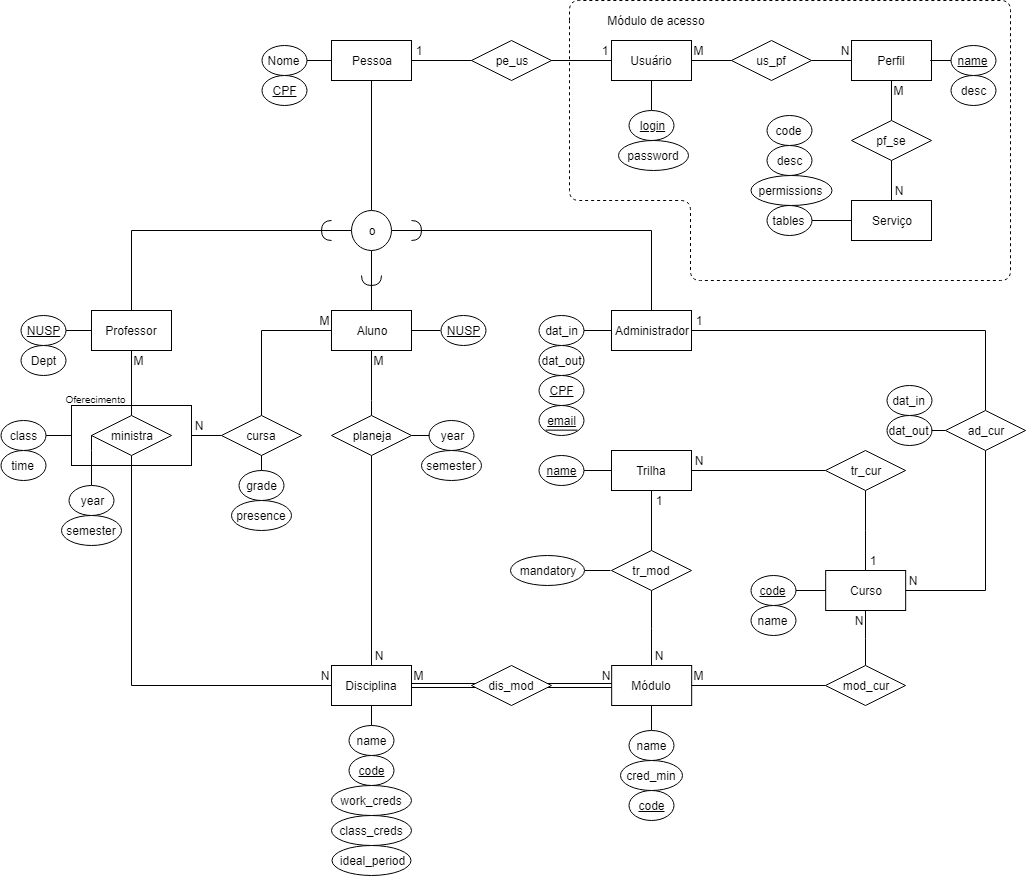
\includegraphics[width=\textwidth]{DER-Completo.png}
    
    \section{Modelo Lógico}
\end{document}